% Opcje klasy 'iithesis' opisane sa w komentarzach w pliku klasy. Za ich pomoca
% ustawia sie przede wszystkim jezyk i rodzaj (lic/inz/mgr) pracy, oraz czy na
% drugiej stronie pracy ma byc skladany wzor oswiadczenia o autorskim wykonaniu.
\documentclass[declaration,shortabstract,polish,inz]{iithesis}

\usepackage[utf8]{inputenc}
\usepackage{listings}
\usepackage{float}
%%%%% DANE DO STRONY TYTUŁOWEJ
% Niezaleznie od jezyka pracy wybranego w opcjach klasy, tytul i streszczenie
% pracy nalezy podac zarowno w jezyku polskim, jak i angielskim.
% Pamietaj o madrym (zgodnym z logicznym rozbiorem zdania oraz estetyka) recznym
% zlamaniu wierszy w temacie pracy, zwlaszcza tego w jezyku pracy. Uzyj do tego
% polecenia \fmlinebreak.
\polishtitle    {Zastosowanie technologii React i Ruby on Rails w tworzeniu aplikacji webowych na przykładzie serwisu blogowego}
\englishtitle   {Application React and Ruby on Rails to create web applications by the example of blog site}

\polishabstract {Celem pracy było opracowanie koncepcji oraz implementacja platformy blogowej łączącej funkcje popularnych serwisów. Do realizacji projektu użyto nowoczesnych rozwiązań. System składa się z dwóch części: aplikacji serwerowej napisanej w języku Ruby z wykorzystaniem Ruby on Rails oraz strony internetowej będącej interfejsem użytkownika zaimplementowanej za pomocą popularnego frameworka React. }

\englishabstract{The purpose of the study was to develop the blog platform that combines the functionality of popular services. Modern solutions were used to implement this project. The system comprises of two parts. Server application was written in Ruby using Ruby on Rails and website that is a user interface was implemented using popular framework React.}
% w pracach wielu autorow nazwiska mozna oddzielic poleceniem \and
\author         {Oskar Sobczyk}
% w przypadku kilku promotorow, lub koniecznosci podania ich afiliacji, linie
% w ponizszym poleceniu mozna zlamac poleceniem \fmlinebreak
\advisor        {dr Leszek Grocholski}
\date          {\today}                     % Data zlozenia pracy
% Dane do oswiadczenia o autorskim wykonaniu
\transcriptnum {281822}                     % Numer indeksu
\advisorgen    {dr. Leszka Grocholskiego} % Nazwisko promotora w dopelniaczu
%%%%%
\usepackage{graphicx}
%%%%% WLASNE DODATKOWE PAKIETY
%
%\usepackage{graphicx,listings,amsmath,amssymb,amsthm,amsfonts,tikz}
%
%%%%% WŁASNE DEFINICJE I POLECENIA
%
%\theoremstyle{definition} \newtheorem{definition}{Definition}[chapter]
%\theoremstyle{remark} \newtheorem{remark}[definition]{Observation}
%\theoremstyle{plain} \newtheorem{theorem}[definition]{Theorem}
%\theoremstyle{plain} \newtheorem{lemma}[definition]{Lemma}
%\renewcommand \qedsymbol {\ensuremath{\square}}
% ...
%%%%%

\begin{document}

%%%%% POCZĄTEK ZASADNICZEGO TEKSTU PRACY

\chapter{Wprowadzenie}
Tematem pracy jest aplikacja internetowa implementująca wybrane funkcje platformy blogowej. Dzisiaj internet jest przepełniony treściami tworzonymi przez jego użytkowników np. poprzez wpisy na portalach społecznościowych lub artykuły na blogach. Jest to atrakcyjna przestrzeń do tworzenia nowych aplikacji pomagających dzielić się treściami. Mimo dużej konkurencji na rynku nadal istnieje zapotrzebowanie na nowe serwisy. Przykładem jest serwis Reddit \cite{reddit} założony w 2005 roku. Dziś jest piątą (według Alexa) najczęściej odwiedzaną stroną w Stanach Zjednoczonych, miesięcznie przyciągającą 330 milionów użytkowników. Na początku jej główną funkcjonalnością była możliwość dzielenia się łączami do stron przez użytkowników oraz głosowania na te strony i ich komentowania. Z czasem, wraz z rozwojem serwisu, użytkownikom dano możliwość dzielenia się nie tylko łączami do innych stron, ale też postami czy obrazkami. Dziś Reddit jest domem dla tysięcy społeczności. Innym przykładem jest powstałe w 2012 roku Medium \cite{medium}. Platforma ta skupia zarówno profesjonalnych dziennikarzy, jak i amatorów. Jej głównym celem jest dostarczenie użytkownikom wartościowych treści w przyjemnej formie. W odróżnieniu od Reddita wspomniana strona skupia się na udostępnianej treści, a nie na interakcjach pomiędzy użytkownikami.

Celem pracy jest stworzenie aplikacji webowej, która łączy możliwość tworzenia rozbudowanych postów zaczerpniętą z Medium z udostępnianiem użytkownikom miejsca do dyskusji na ich temat podobnie jak w Reddicie.

W wyborze zestawu narzędzi do realizacji implementacji pracy kierowałem się tym, aby zawierał on jak najwięcej nowych, wykorzystywanych na rynku komercyjnym rozwiązań, co pozwoliłoby mi poszerzyć moje umiejętności. W wyniku realizacji celu pracy powstała aplikacja składająca się z dwóch podstawowych części: \textbf{blogger-frontend}, \textbf{blogger-backend}.


\chapter{Wymagania}

Pierwsze blogi powstały w późnych latach 90. Były prostymi, statycznymi stronami WWW aktualizowanymi ręcznie. Wpisy były wyświetlane użytkownikowi w odwrotnej chronologicznej kolejności. Wraz z upływem czasu i wzrostem popularności internetowych dzienników powstały specjalne serwisy oraz oprogramowanie służące do ich obsługi. Pozwoliło to na prowadzenie własnego bloga przez przeciętnego użytkownika internetu. Dzisiaj najpopularniejszą odmianą są mikroblogi – strony umożliwiające użytkownikom dzielenie się krótkimi, kilku zdaniowymi przemyśleniami lub obrazkami, np. Twitter \cite{twitter}, Facebook \cite{facebook}, Wykop.pl \cite{wykop}. Poniżej opisano wymagania funkcjonalne i niefunkcjonalne wytwarzanego systemu.

\subsubsection{Wymagania funkcjonalne}

\begin{itemize}
    \item Niezalogowany użytkownik może: 
    \begin{itemize}
         \item zalogować się na istniejące konto;
         \item utworzyć nowe konto;
         \item przeglądać listę postów;
         \item przeglądać post wraz z jego komentarzami;
         \item przeglądać listę kategorii – posty w danej kategorii.
    \end{itemize}
    \item Zalogowany użytkownik może:
        \begin{itemize}
            \item wylogować się;
            \item pisać nowe posty
            \item pisać komentarze;
            \item przeglądać listę powiadomień.
        \end{itemize}
\end{itemize}

\subsubsection{Wymagania niefunkcjonalne}
\begin{itemize}
    \item prosty interfejs użytkownika,
    \item bezpieczny system kont dla użytkowników,
    \item rozszerzalność,
    \item wykorzystanie narzędzi do statycznej analizy kodu,
    \item zastosowanie narzędzi do ciągłej integracji podczas wytwarzania kodu,
    \item działanie projektu w systemie Linux.
    
\end{itemize}

% \subsection{Wnioski}-
\chapter{Część dla programisty}
\section{Architektura aplikacji}
Aplikacja jest napisana w architekturze klient-serwer, podczas jej tworzenia wykorzystano wzorzec separacji zagadnień (ang. \textit{separation of concerns}, SoC). Pozwoliło to na podzielenie serwisu na dwie części. Pierwszą jest warstwa dostępu do danych napisana w języku Ruby \cite{ruby} z wykorzystaniem Ruby on Rails \cite{ror}. Odpowiada ona za przechowywanie danych w bazie danych PostgreSQL \cite{postgre} oraz za ich udostępnianie za pomocą API. Drugą częścią jest warstwa prezentacji, która wykorzystuje JavaScript oraz framework React \cite{react} w celu prezentacji danych. Taki podział pozwala na niezależny rozwój każdej części aplikacji.

\section{Uruchomienie aplikacji}

\subsection{Backend}
Wymagane oprogramowanie do uruchomienia części serwerowej:
        \begin{itemize}
            \item Ruby w wersji 2.6.2,
            \item Bundler \cite{bundler} w wersji 1.17,
            \item Foreman \cite{foreman} w wersji 0.85.0,
            \item Pozostałe zależności z pliku \textit{Gemfile},
            \item PostgreSQL w wersji 11.3,
            \item Redis \cite{redis} w wersji 5.0.5.
        \end{itemize}

Oto czynności, które trzeba wykonać, aby zainstalować część serwerową:
\begin{enumerate}
    \item W katalogu \textit{blogger-backend} poleceniem \textit{bundle install} zainstalować dodatkowe biblioteki.
    \item Poleceniem \textit{rake db:create} utworzyć bazę danych.
    \item Wykonać migracje do bazy danych poleceniem \textit{rake db:migrate}.
    \item Wypełnić bazę danych przykładowymi danymi peleceniem \textit{rake db:seed}.
    \item Poleceniem \textit{foreman start -f Procfile.dev} uruchomić serwer.
\end{enumerate}

\subsection{Frontend}
Wymagane oprogramowanie do uruchomienia frontendu:
    \begin{itemize}
        \item Yarn \cite{yarn} w wersji 1.13.0,
        \item Zależności znajdujące się w pliku \textit{package.json}.
    \end{itemize}

Oto czynności, które trzeba wykonać, aby uruchomić frontend:
\begin{enumerate}
    \item W folderze \textit{blogger-frontend} poleceniem \textit{yarn} zainstalować brakujące pakiety.
    \item Poleceniem \textit{yarn start} uruchomić serwer deweloperski, jego domyślny adres \textit{localhost:3001}.
\end{enumerate}

\section{Backend}
\subsection{Ruby on Rails}
Część serwerowa została napisana z wykorzystaniem frameworka Ruby on Rails. Powstał on w 2005 roku \cite{rorwiki} jako narzędzie do szybkiego tworzenia aplikacji webowych. Głównymi strategiami projektowymi są „Convention Over Configuration” \cite{coc} oraz DRY („Don’t repeat yourself”) \cite{dry}. Dzięki temu programista już po zainicjowaniu projektu uzyskuje domyślną strukturę oraz konfigurację pozwalającą ominąć żmudny proces ręcznego definiowania ustawień. Już w momencie powstania Ruby on Rails oferował wiele innowacyjnych funkcji, takich jak generowanie tabel w bazie danych na podstawie modeli, scaffolding oraz system migracji. Dzisiaj napędza takie serwisy jak GitHub, Aribnb, Kickstarter, a inspirację nim możemy znaleźć w wielu innych frameworkach, np. Django \cite{django}, Sails.js \cite{sails}.

\begin{figure}[H]
    \centering
    \begin{minipage}[b]{0.4\textwidth}
        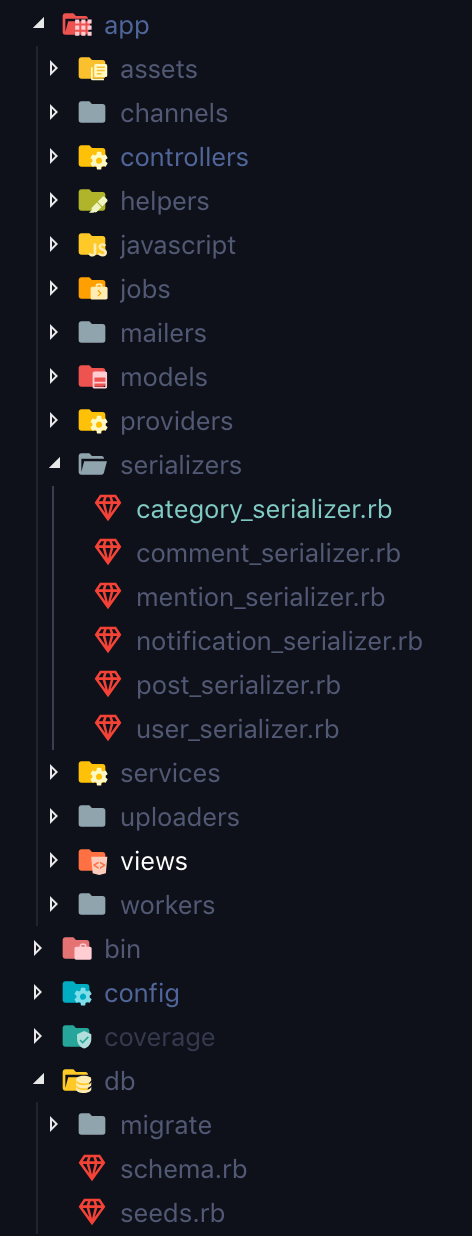
\includegraphics[width=\textwidth]{images/serwer1.png}
        \caption{Struktura części serwerowej, cz. 1}
        \label{fig:struktura_serwer1}
    \end{minipage}
    \hfill
    \begin{minipage}[b]{0.4\textwidth}
        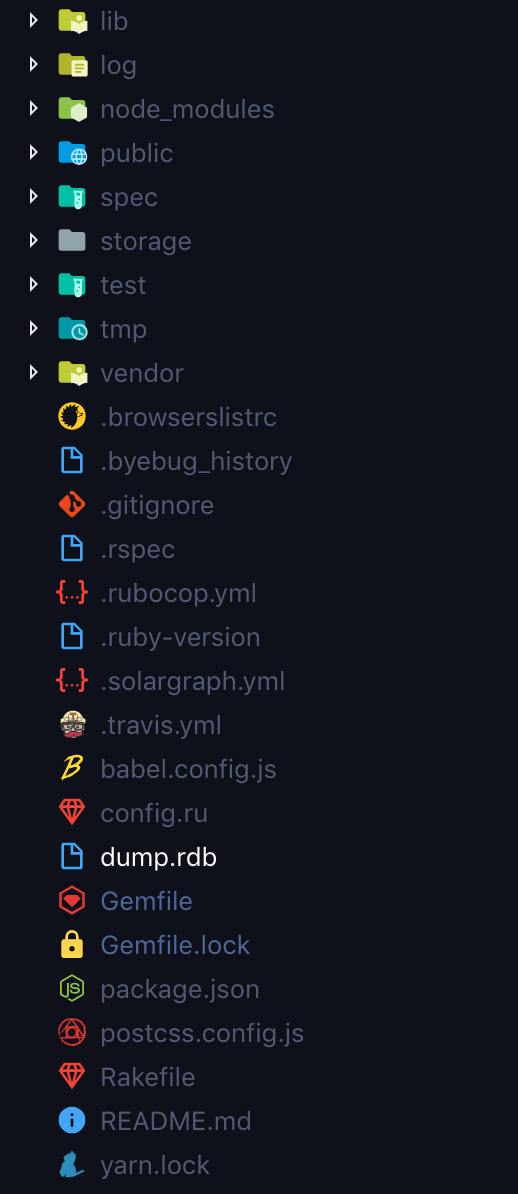
\includegraphics[width=\textwidth]{images/serwer2.png}
        \caption{Struktura części serwerowej, cz. 2}
        \label{fig:struktura_serwer2}
    \end{minipage}
\end{figure}
\subsection{Struktura backendu}
Struktura części serwerowej przedstawiona na rysunkach \ref{fig:struktura_serwer1} i \ref{fig:struktura_serwer2} powstała w wyniku działania wbudowanego w Ruby on Rails generatora. Utworzył on minimalną konfigurację potrzebną do rozpoczęcia pracy. Framework implementuje architekturę \textbf{MVC (Model-Widok-Kontroler)} \cite{rortutorial}. Zakłada ona podział na trzy główne części. Model jest odpowiedzialny za zarządzanie danymi oraz implementacje logiki biznesowej. Widok ma za zadanie prezentację modelu za pomocą ustalonego formatu. Natomiast kontroler przyjmuje żądania od użytkownika i wykonuje operacje na modelach. Najważniejszą częścią projektu jest katalog \textit{app} zawierający wszystkie komponenty aplikacji. W podkatalogu \textit{app/controllers} umieszczono kontrolery odpowiadające za nadanie sensu żądaniom przychodzącym do API oraz za wygenerowanie poprawnej odpowiedzi (rys. \ref{fig:kontroler}). W nazwie każdego kontrolera zawarta jest informacja, na jakim modelu on operuje. W \textit{app/services} znajdują się klasy serwisów, które implementują interakcje użytkownika z aplikacją. Pozwala to na wyodrębnienie logiki biznesowej z kontrolerów. Konfiguracje do serializera odpowiedzialnego za przekształcanie instancji modeli na format JSON znajdują się w folderze \textit{app/serializers}. Definicje modeli (rys. \ref{fig:model}) zlokalizowane są w folderze \textit{app/models}. Katalog \textit{db} zawiera aktualny schemat bazy danych, co umożliwia przenoszenie bazy pomiędzy komputerami oraz migrację, czyli zestaw plików napisany w Ruby DSL pozwala na zmianę schematu bazy danych bez potrzeby pisania ręcznie poleceń SQL.
\begin{figure}
    \centering
    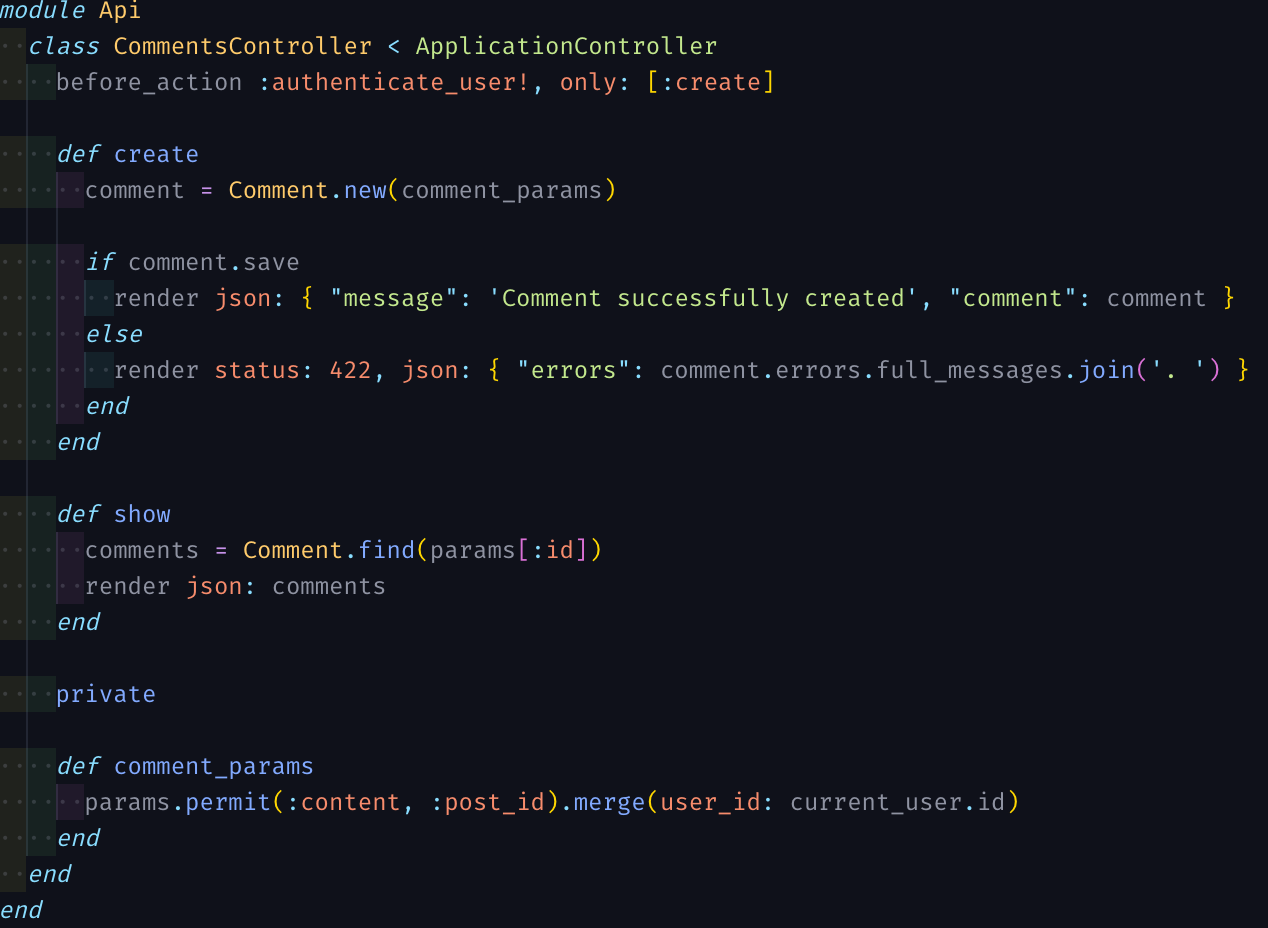
\includegraphics[width=\textwidth]{images/kontroler.png}
    \caption{Kod przykładowego kontrolera}
    \label{fig:kontroler}
\end{figure}
\begin{figure}
    \centering
    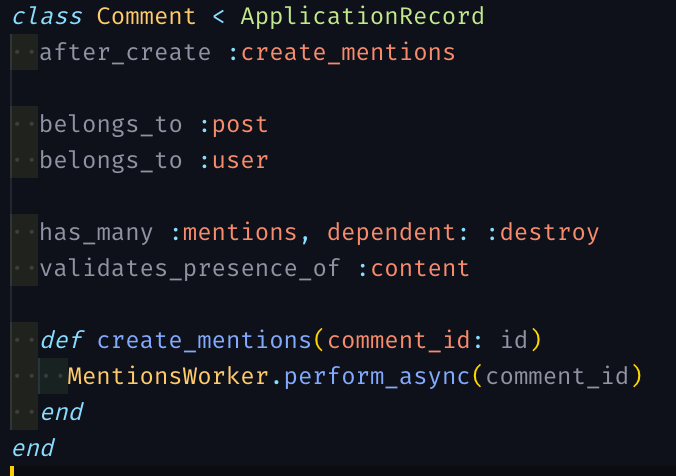
\includegraphics[width=0.5\textwidth]{images/comment_model.png}
    \caption{Kod przykładowego modelu}
    \label{fig:model}
\end{figure}


\subsection{Baza danych}
Jako system przechowywania danych wybrano PostgreSQL. Jest to otwartoźródłowy silnik do zarządzania relacyjnymi bazami danych. Charakteryzuje się wysoką kompatybilnością ze standardem SQL:2011 \cite{sql2011}, zgodnością z ACID \cite{acid} (ang. \textit{Atomicity, Consistency, Isolation, Durability}) oraz niezawodnością. Ruby on Rails w domyślnej konfiguracji zapewnia wsparcie dla Postgresa. Pozwala to na zastosowanie systemu migracji, który wraz z rozbudową aplikacji odpowiednio modyfikuje istniejący schemat bazy danych.


\subsubsection{Schemat bazy danych}
Baza danych (rys. \ref{fig:erd_diagram}) składa się z następujących tabel: 
\begin{itemize}
    \item \textbf{user} - zawiera między innymi takie informacje jak imię, e-mail, hasło. Jest wykorzystywana podczas uwierzytelniania.
    \item \textbf{post} - podstawowy typ danych w platformie blogowej. Składa się z tytułu, zawartości oraz łącza do miniaturki.
    \item \textbf{comment} - przechowuje zawartość komentarzy.
    \item \textbf{like} - odpowiada za przechowywanie głosów użytkowników.
    \item \textbf{mention} - gromadzi dane z systemu wspomnień. Dla każdej wspomnianej osoby w komentarzu przechowuje wpis z identyfikatorem użytkownika oraz komentarza, co pozwala na szybkie znalezienie zarówno osób skojarzonych z wpisem, jak i postów przypisanych danej osobie.
    \item \textbf{notification} - odpowiada za powiadomienia. Dzięki polimorficznym asocjacjom możliwa jest rozbudowa tego systemu wraz z rozwojem aplikacji. Dla każdego wpisu w tabeli pamiętany jest zarówno identyfikator powiązanego obiektu, jak i jego typ. Pozwala to, aby jedna tabela zawierała odniesienia do wielu tabel.
\end{itemize}
\begin{figure}[H]
    \centering
    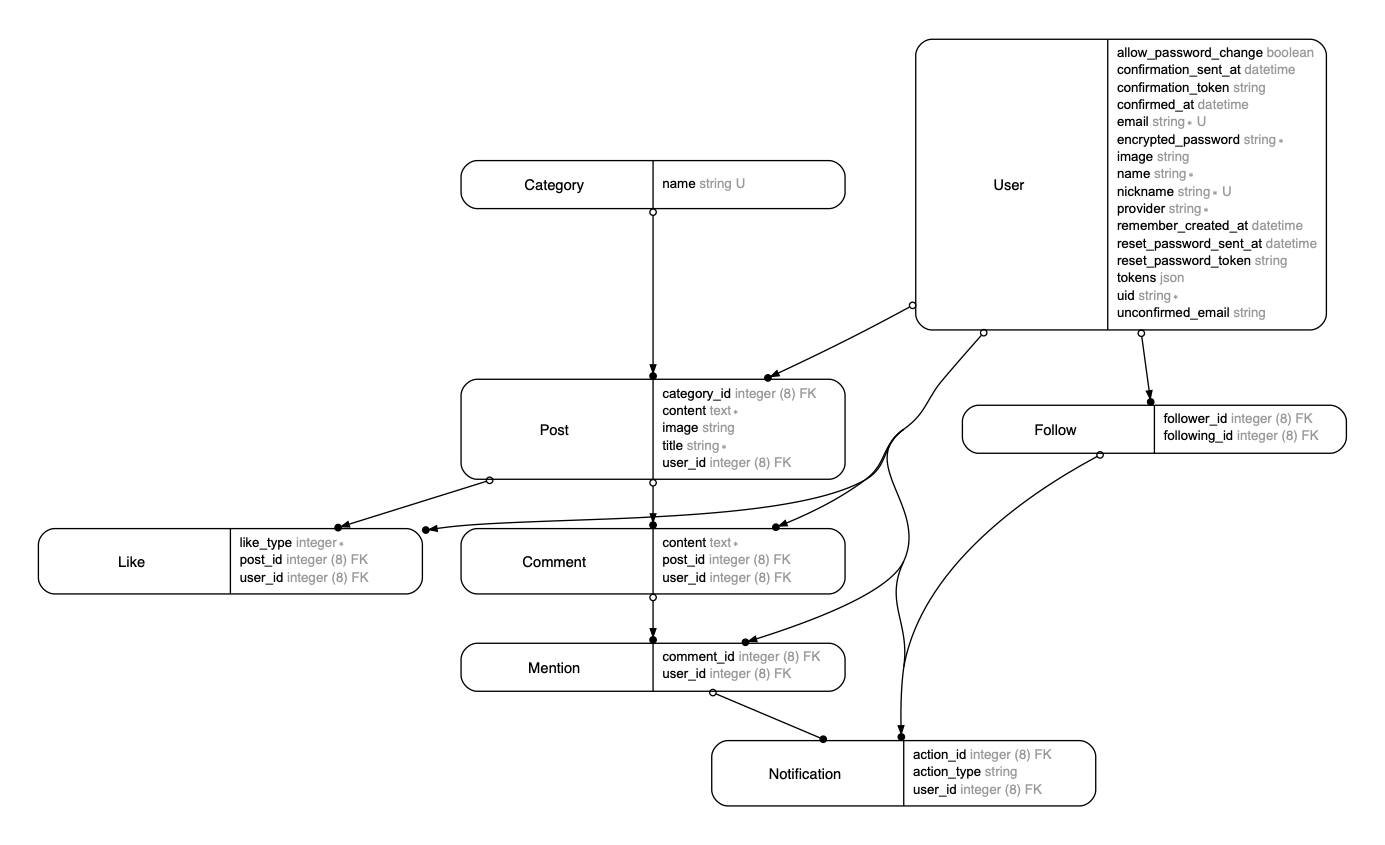
\includegraphics[width=\textwidth]{images/erd.png}
    \caption{Schemat ERD bazy danych}
    \label{fig:erd_diagram}
\end{figure}

\subsection{Redis}
W projekcie wykorzystano bibliotekę Sidekiq \cite{sidekiq} do przetwarzania zadań w tle. Do jej poprawnego działania wymagany jest Redis. Jest to nierelacyjna baza danych klucz-wartość przechowywana w pamięci głównej komputera. Dzięki temu charakteryzuje się wysoką wydajnością.

\begin{figure}[H]
    \centering
    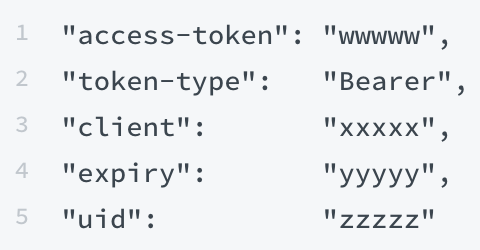
\includegraphics{images/token.png}
    \caption{Struktura tokenu}
    \label{fig:token2}
\end{figure}
\subsection{Uwierzytelnianie}
Aby ograniczyć dostęp do wybranych funkcjonalności API, wykorzystano system uwierzytelniania bazujący na tokenie. Użytkownik po pomyślnym zalogowaniu się otrzymuje w nagłówku odpowiedzi od serwera token (rys \ref{fig:token2}). Jego dołączenie do nagłówków późniejszych zapytań kierowanych do chronionej części API będzie obligatoryjne. Pozwoli to na identyfikację użytkownika. W przypadku jego braku serwer zwróci w odpowiedzi błąd. W celu zwiększenia bezpieczeństwa serwisu, podczas każdego zapytania zostaje wygenerowany nowy token, natomiast stary zostaje unieważniony (rys. \ref{fig:token}).

\begin{figure}[H]
    \centering
    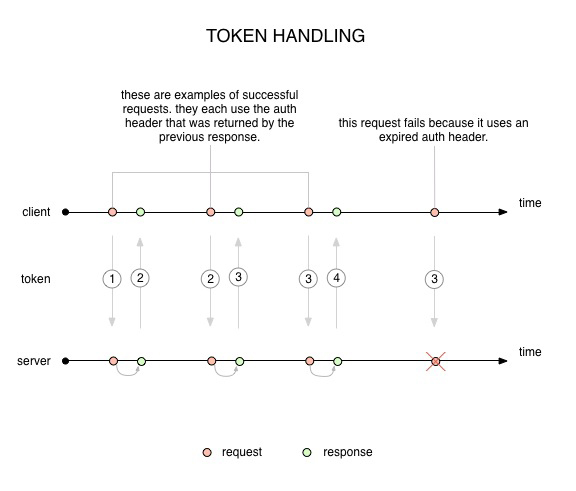
\includegraphics[width=0.9\textwidth]{images/token-update-detail.jpg}
    \caption{Proces obsługi tokenu \cite{token}}
    \label{fig:token}
\end{figure}

\subsection{Ciągła integracja}
W procesie wytwarzania oprogramowania zastosowano technikę ciągłej integracji (z ang. \textit{continuous integration}) \cite{ci} z wykorzystaniem serwisu Travis CI \cite{travis}. Każdy zestaw zmian wysyłany do repozytorium GIT wyzwala proces przeprowadzenia testów oraz statycznej analizy kodu. Taka praktyka przyśpiesza wykrywanie błędów oraz wspomaga egzekwowanie wytycznych dotyczących stylu kodu.

\section{Frontend}

\subsection{React}
Interfejs udostępniany użytkownikowi został napisany z wykorzystaniem Reacta. Jest to biblioteka JavaScript utworzona w 2013 roku \cite{reactwiki} i utrzymywana przez Facebook. Dziś jest jednym z najpopularniejszych frameworków do tworzenia interfejsów użytkownika. Jego główną cechą charakterystyczną jest budowanie złożonych projektów za pomocą wielu mniejszych, wyizolowanych części nazywanych komponentami. Są to klasy lub funkcje, które mogą przyjmować jako wejście właściwości (\textit{props}), a zwracają opis, jak dany komponent powinien zostać wyrenderowany przez przeglądarkę. Dodatkowo React pozwala na to, aby komponenty posiadały stan, czyli zestaw danych, które można zmieniać. Biblioteka ta umożliwia również dynamiczne modyfikowanie HTML-a bez potrzeby odświeżania stron. Istnieje możliwość wykorzystania Reacta na urządzeniach mobilnych za pomocą React Native \cite{reactnative}.

\subsection{Ant Design}
Bardzo ważnym elementem aplikacji udostępnianej klientowi jest jej wygląd, dlatego aby całość aplikacji prezentowała się spójnie, zdecydowano się zastosować wytyczne Ant Design \cite{ant} oraz ich implementację za pomocą biblioteki \textit{antd} zawierającej zestaw komponentów Reacta. Znacznie zmniejszyło to czas potrzebny na dodawanie stylów do nowych komponentów i pozwoliło skupić się na implementacji nowych funkcjonalności.

\begin{figure}[H]
    \centering
    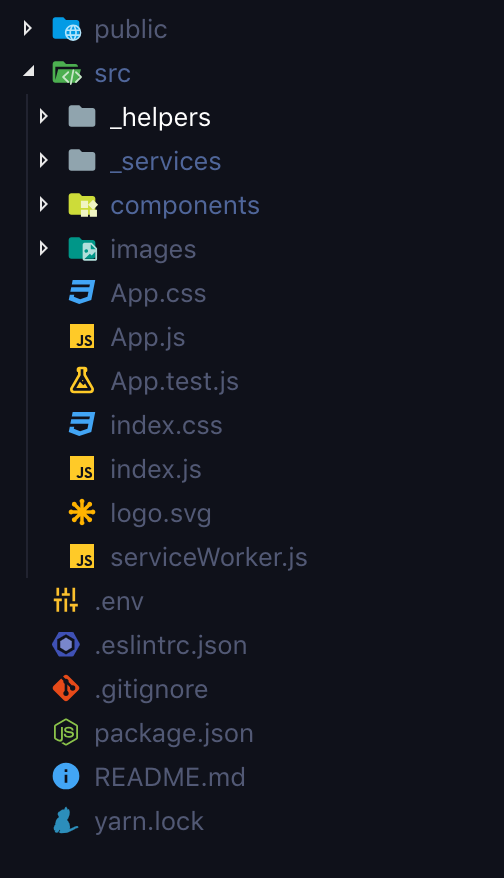
\includegraphics[height=10cm]{images/forontend.png}  
    \caption{Struktura projektu}
    \label{fig:frontend_struct}
\end{figure}
\subsection{Struktura projektu}
Projekt zainicjowano za pomocą narzędzia \textit{create-react-app} \cite{cra} dostarczanego przez Facebook. Tworzy ono gotowe, skonfigurowane środowisko umożliwiające natychmiastowe rozpoczęcie pracy nad aplikacją. Kod aplikacji podzielono w następujących folderach (rys. \ref{fig:frontend_struct}):
\begin{itemize}
    \item \textbf{\textunderscore helpers} - zawiera pomocnicze funkcje nieprzypisane do konkretnego komponentu.
    \item \textbf{\textunderscore services} - znajdują się tu funkcje odpowiedzialne za interakcję z API.
    \item \textbf{componets} - jest to najważniejszy folder. To w nim umieszczone są wszystkie komponenty odpowiedzialne za wygląd i działanie aplikacji. Dodatkowo komponenty zostały podzielone ze względu na swoje zastosowanie.
\end{itemize}

Punktem wejścia do aplikacji jest \textit{App.js} (rys. \ref{fig:app.js}), gdzie został zdefiniowany komponent odpowiedzialny za routing. Wykorzystano do tego celu bibliotekę \textit{react-router}\cite{reactrouter} i komponenty \textit{Route}, które zwracają wartość, tylko jeśli adres URL jest zgodny ze zdefiniowanym w path. W następnym kroku zostanie wyrenderowany konkretny komponent. React pozwala programiście na budowanie ich za pomocą funkcji lub klas. Od niedawna oba sposoby posiadają zbliżone funkcjonalności. Przykładowy komponent przedstawiony na rysunku \ref{fig:komponent1} odpowiedzialny jest za wyświetlanie listy postów. W pierwszych liniach deklarowany jest stan za pomocą funkcji \textit{useState}. Następnie znajduje się funkcja \textit{useEffect} \cite{hooks}, która jest odpowiednikiem metod cyklu życia z komponentów klasowych. W tym wypadku odpowiada ona za pobranie listy postów z serwera oraz zapisanie ich do stanu. Ostatnią czynnością komponentu jest zwrócenie obiektu, który ma zostać wyrenderowany.

\begin{figure}[H]
    \centering
    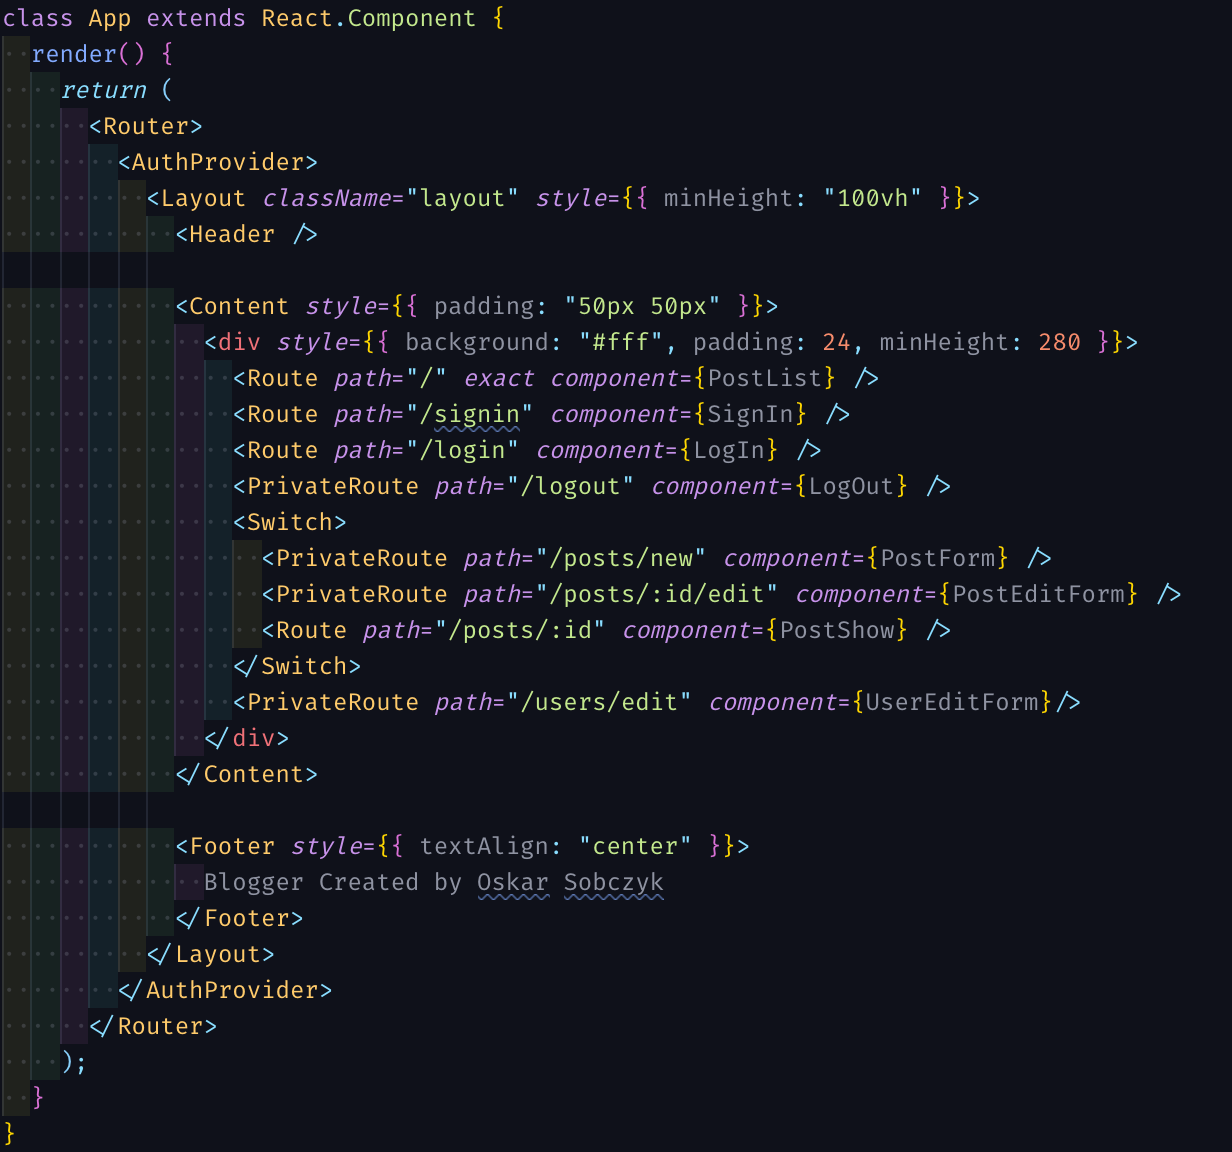
\includegraphics[width=\textwidth]{images/appjs.png}
    \caption{Plik App.js}
    \label{fig:app.js}
\end{figure}

\begin{figure}
    \centering
    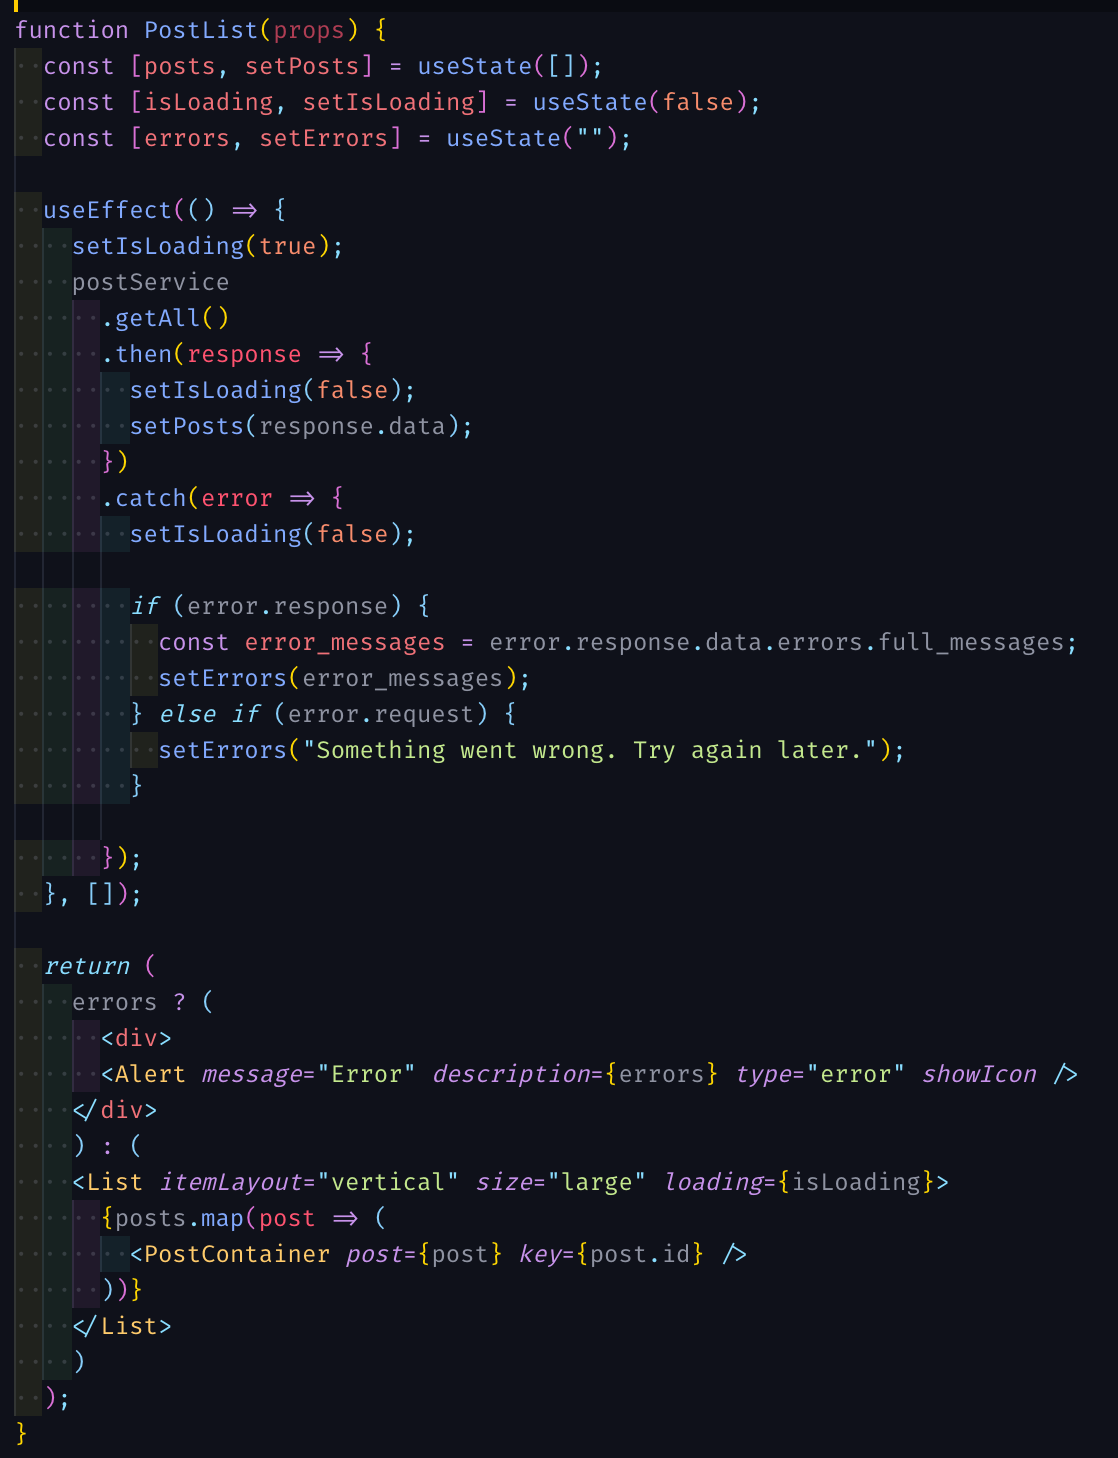
\includegraphics[width=\textwidth]{images/komponent1.png}
    \caption{Przykładowy komponent}
    \label{fig:komponent1}
\end{figure}

\chapter{Część dla użytkownika}
\section{Dostęp do systemu}
Blogger jest platformą blogową pozwalającą użytkownikowi dodawać wpisy w jednej z predefiniowanych kategorii. Mogą oni również wchodzić w interakcję między sobą poprzez dyskusje pod wpisami lub system ich oceniania. Aby móc korzystać z tych funkcji, wystarczy utworzyć i zweryfikować konto za pomocą e-maila.

Działający system jest dostępny pod adresem \url{https://young-sea-15783.herokuapp.com/}. Aby móc korzystać ze wszystkich możliwości serwisu, należy założyć konto i potwierdzić je, klikając w link otrzymany drogą e-mailową. Dostępne jest również konto testowe – e-mail: \textit{test@test.pl}, hasło: \textit{test123}.

\section{Demonstracja aplikacji}
Serwis można podzielić na dwa moduły: jeden jest dostępny dla każdego użytkownika, drugi – tylko dla zalogowanego.
\subsection{Niezalogowany użytkownik}
\subsubsection{Strona główna}
Użytkownik po wpisaniu adresu aplikacji w przeglądarce zostanie przekierowany na stronę główną (rys. \ref{fig:main_page}), na której będzie mógł przeglądać listę wszystkich postów, jakie zostały utworzone. Każdy z nich jest reprezentowany przez przeglądowy opis, na który składają się: tytuł, skrócona treść wpisu oraz graficzna miniaturka. Użytkownik może zostać przeniesiony do szczegółowego widoku wpisu po kliknięciu w jeden z nich.

\begin{figure}[H]
    \centering
    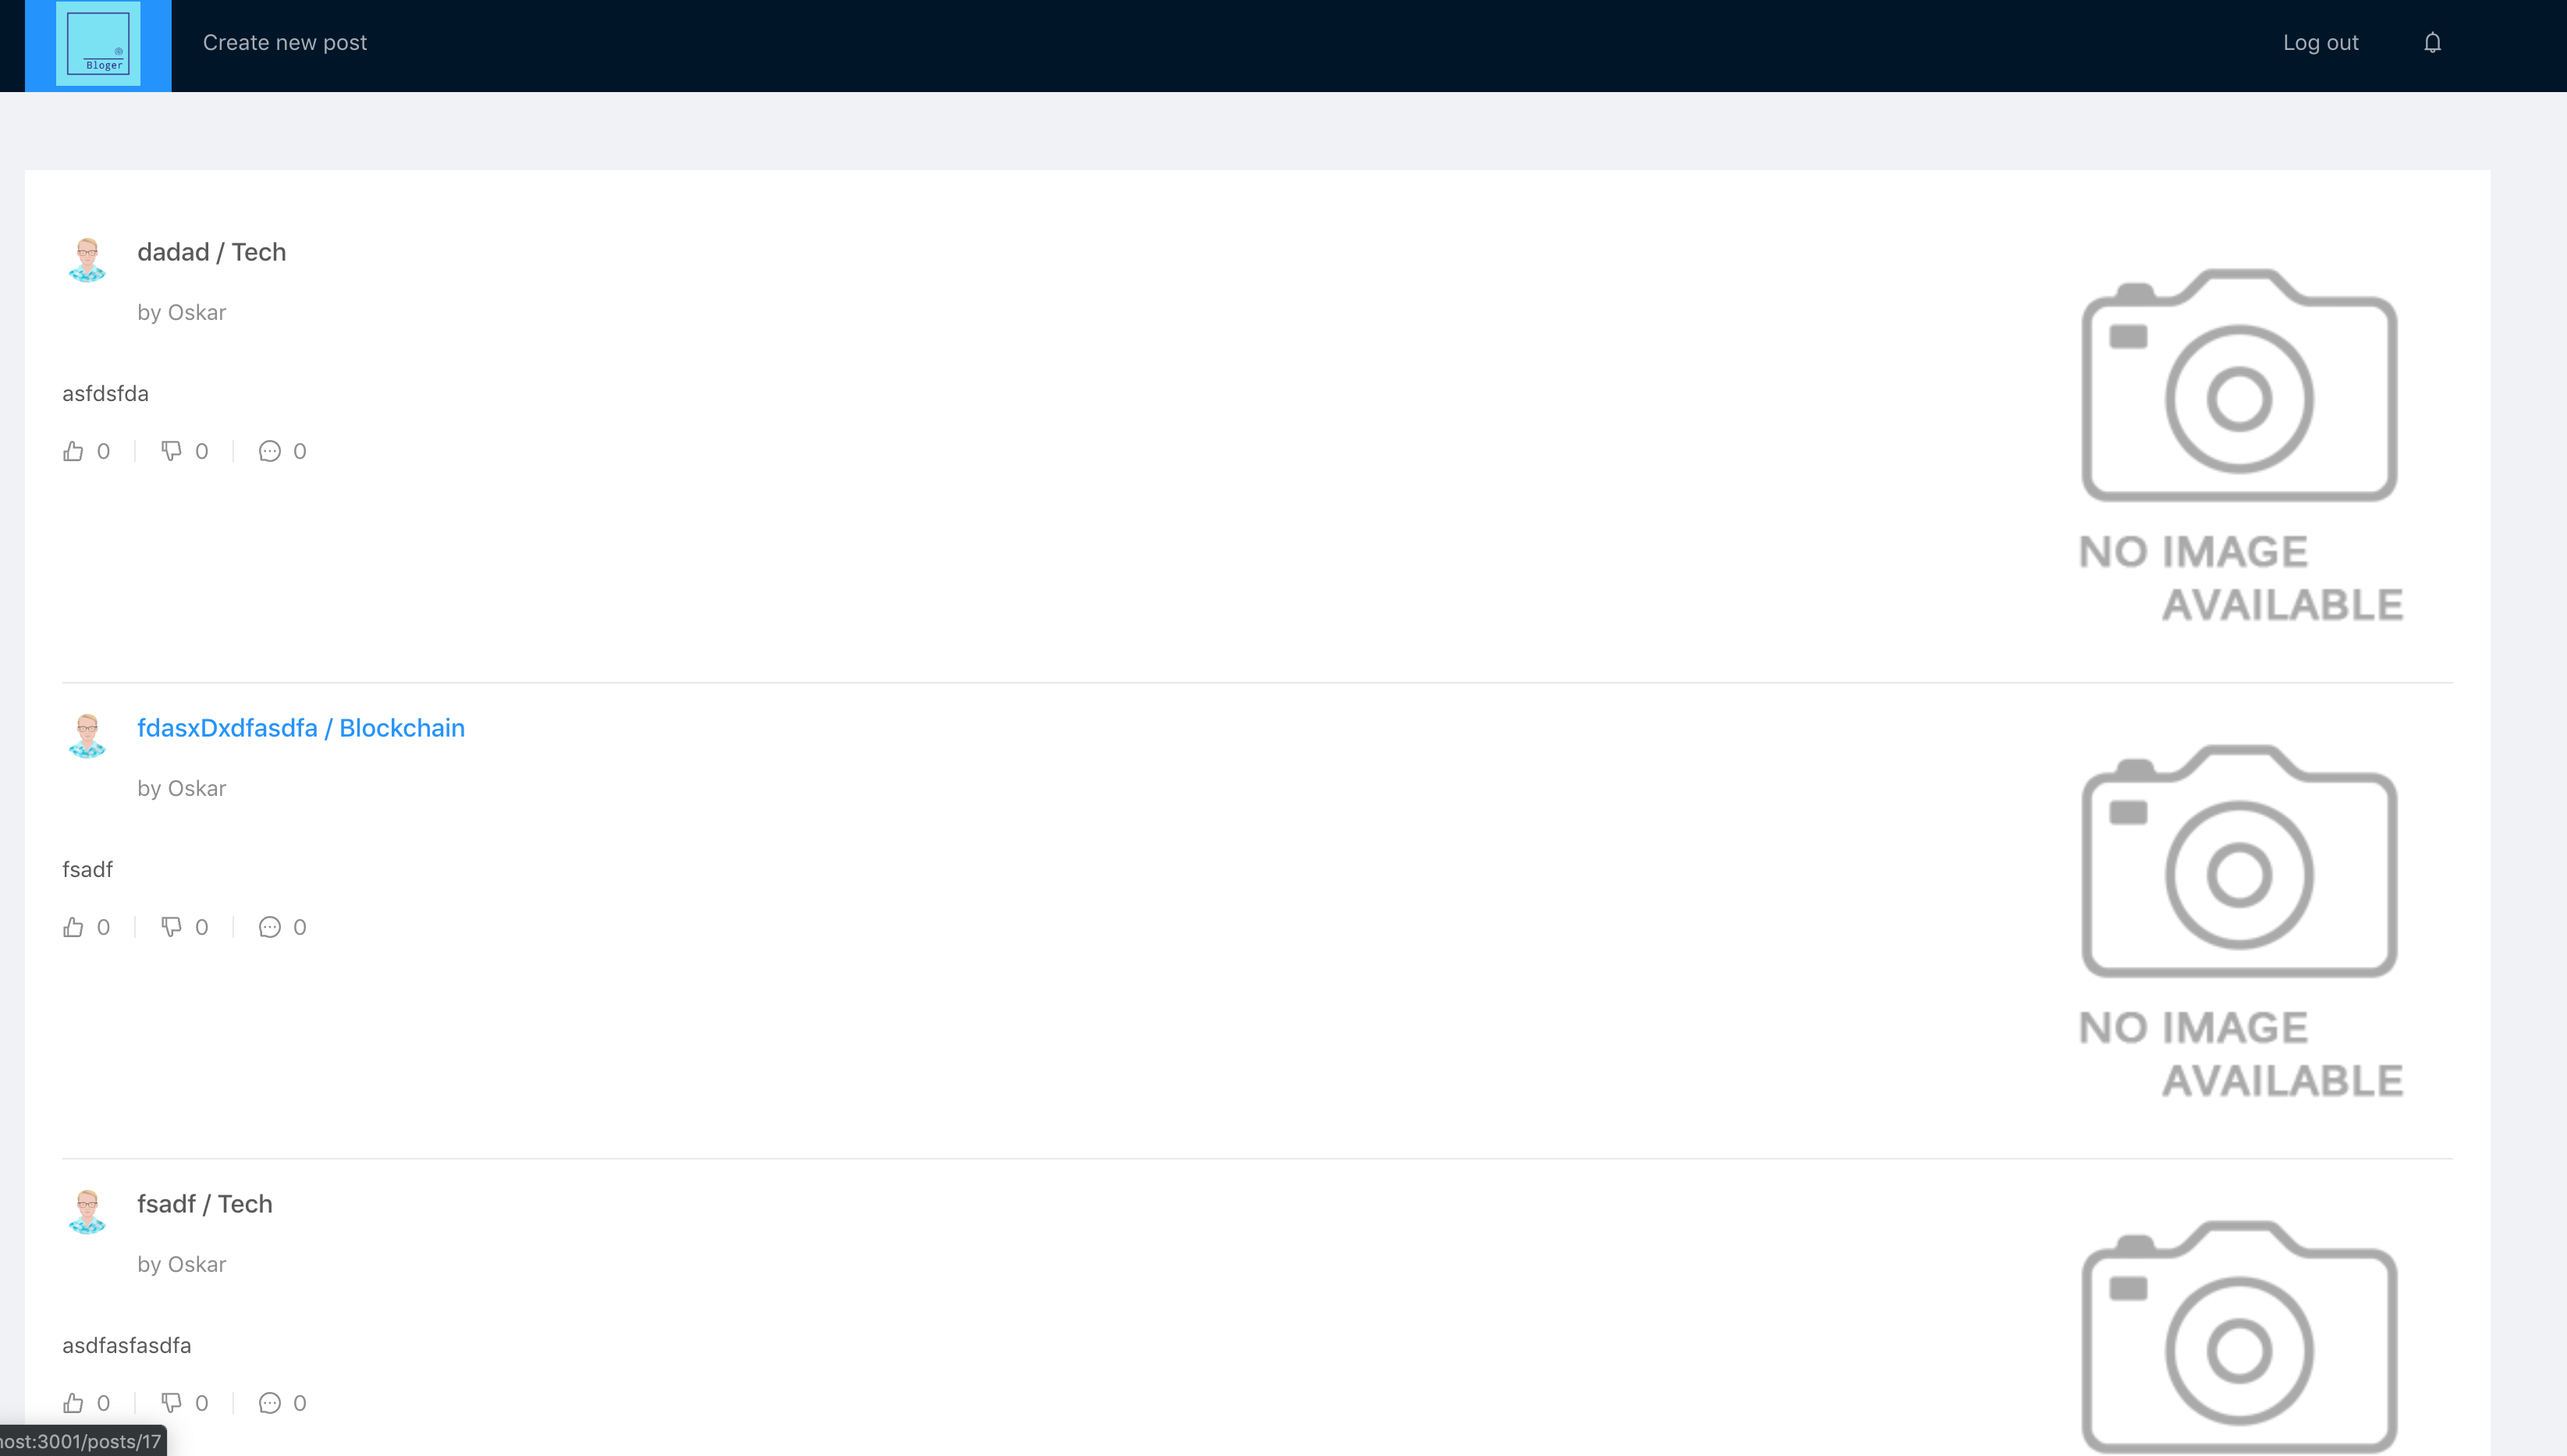
\includegraphics[width=\textwidth]{images/stronaglowna.png}
    \caption{Ekran strony głównej}
    \label{fig:main_page}
\end{figure}

\subsubsection{Szczegółowy widok wpisu}
W tym widoku (rys. \ref{fig:post_view}) użytkownik ma dostęp do pełnej treści wpisu oraz komentarzy.

\begin{figure}[H]
    \centering
    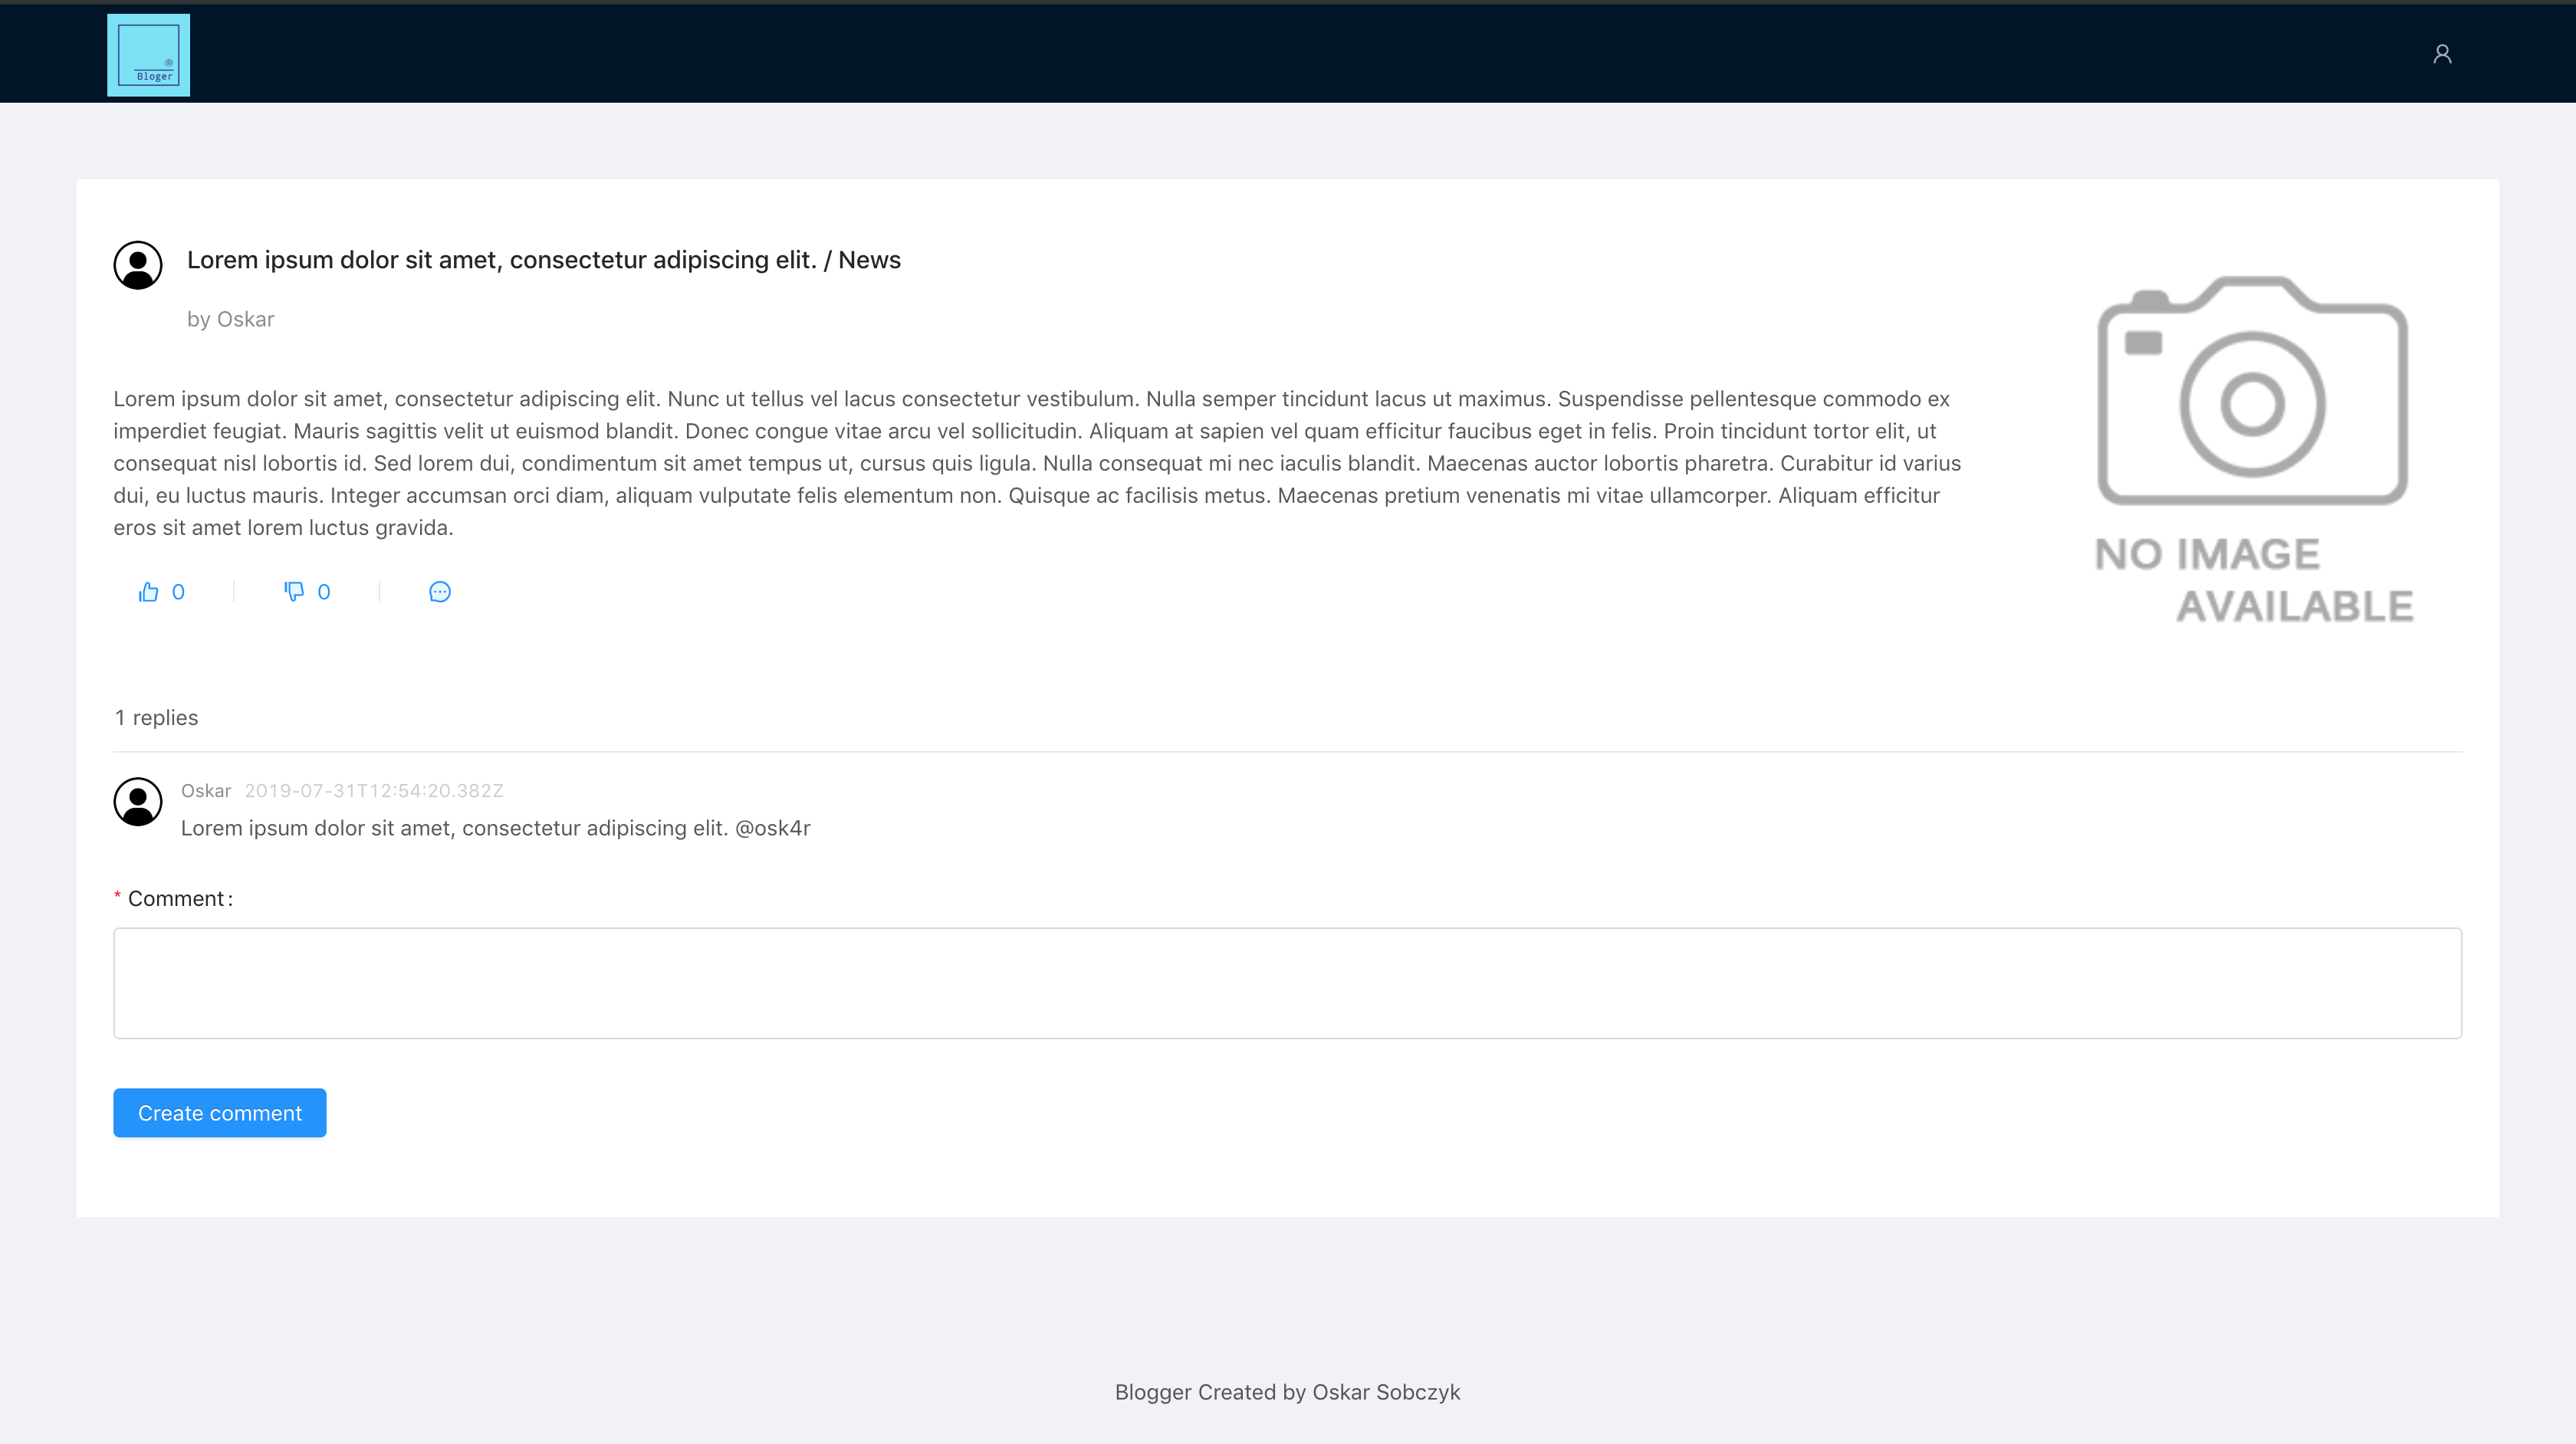
\includegraphics[width=\textwidth]{images/widok_postu.png}
    \caption{Ekran widoku szczegółowego}
    \label{fig:post_view}
\end{figure}

\subsubsection{Rejestracja nowego użytkownika}
Aby zarejestrować się w serwisie (rys. \ref{fig:register}), należy podać imię, nick, e-mail, hasło. Opcjonalnie użytkownik może dodać swój awatar. Po wysłaniu formularza na podany wcześniej adres poczty zostanie wysłany link aktywujący konto.

\begin{figure}[H]
    \centering
    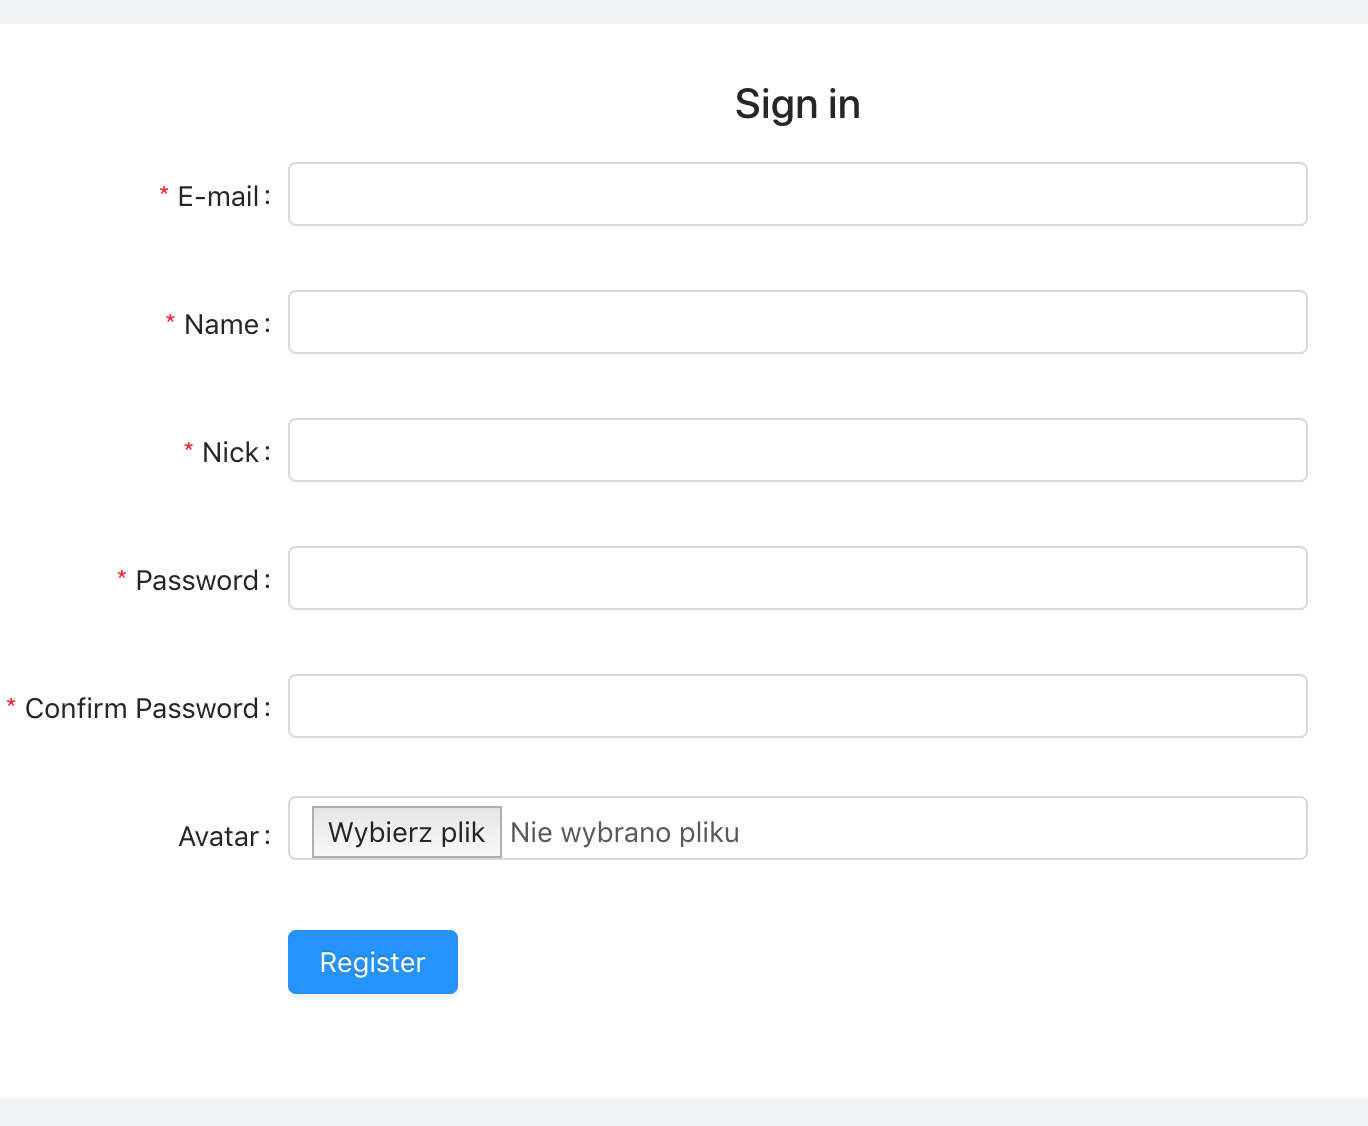
\includegraphics[width=\textwidth]{images/rejestracja.png}
    \caption{Formularz rejestracji nowego użytkownika}
    \label{fig:register}
\end{figure}

\subsubsection{Logowanie}
Aby móc korzystać ze wszystkich możliwości serwisu, wymagane jest logowanie (rys. \ref{fig:login}). Możliwe jest ono tylko po wcześniejszej aktywacji konta. W tym celu należy podać adres e-mail oraz hasło.

\begin{figure}[H]
    \centering
    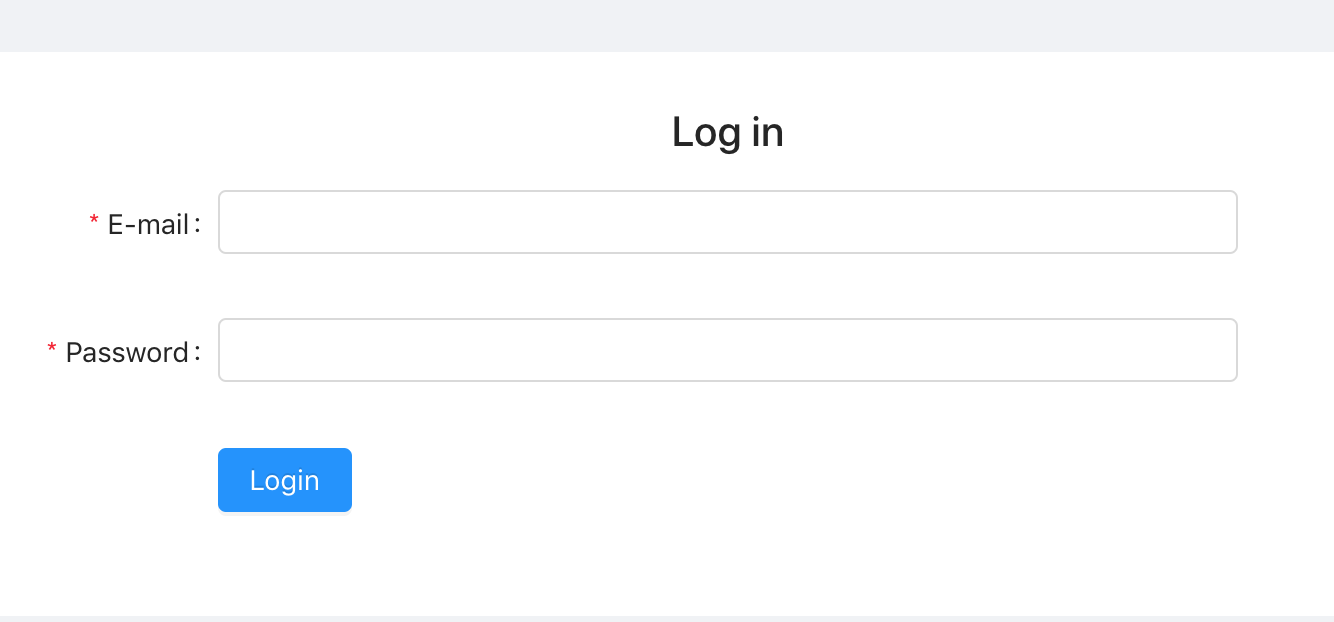
\includegraphics[width=\linewidth]{images/logowanie.png}
    \caption{Formularz logowania}
    \label{fig:login}
\end{figure}

\subsection{Zalogowany użytkownik}

\subsubsection{Dodawanie wpisów}
Zalogowany użytkownik może dodawać wpisy do serwisu. Aby to zrobić, musi kliknąć przycisk znajdujący się w nagłówku strony \textit{Create new post}, następnie zostanie przekierowany do odpowiedniego formularza. Tam do wypełnienia będzie miał takie pola jak: tytuł, treść, kategoria oraz miniaturka. Po wysłaniu i walidacji formularza wpis zostanie utworzony, a użytkownik przekierowany na jego stronę.

\subsubsection{Ocenianie wpisów}
Każdy zalogowany użytkownik ma możliwość oceniania innych użytkowników. Wystarczy, że kliknie w łapkę w dół lub w górę przy danym poście (rys. \ref{fig:like}).
\begin{figure}[H]
    \centering
    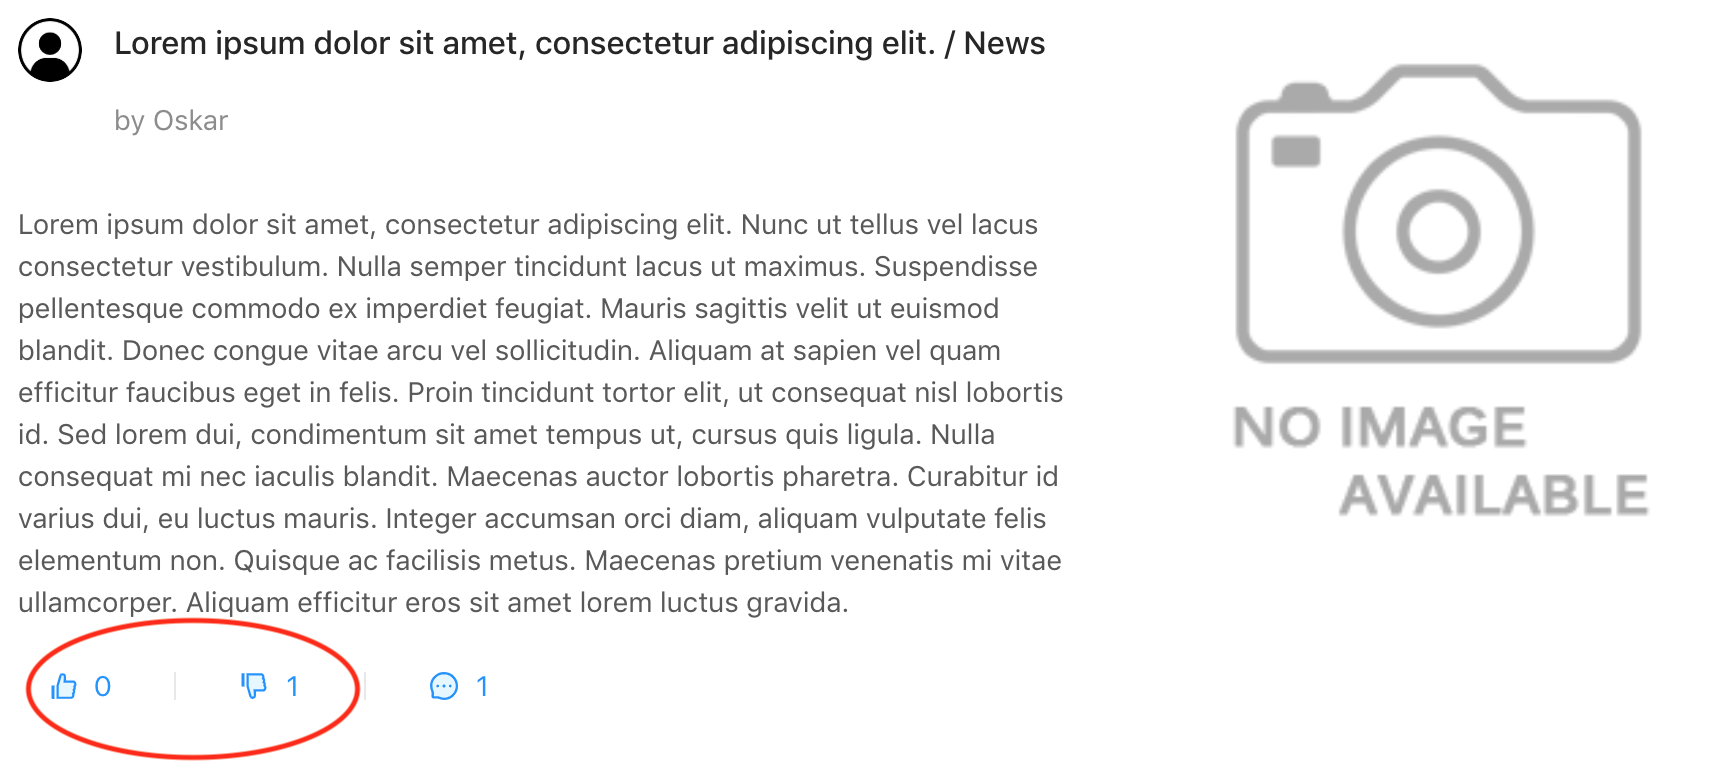
\includegraphics[width=\linewidth]{images/like.png}
    \caption{Ekran modułu oceniania}
    \label{fig:like}
\end{figure}

\subsubsection{Komentarze}
Dla zalogowanych użytkowników udostępniona została funkcja dyskusji na temat wpisów za pomocą komentarzy (rys. \ref{fig:comment}). Dodawanie nowych komentarzy jest możliwe z wykorzystaniem formularza dostępnego w szczegółowym widoku wpisu. Dodatkowo w system komentarzy wbudowany jest system „wołania”. Aby „zawołać” innego użytkownika w treści komentarza, należy jego nick poprzedzić symbolem \textit{@}. W ten sposób wspomniany użytkownik otrzyma powiadomienie o naszej aktywności (rys. \ref{fig:notification}).

\begin{figure}[H]
    \centering
    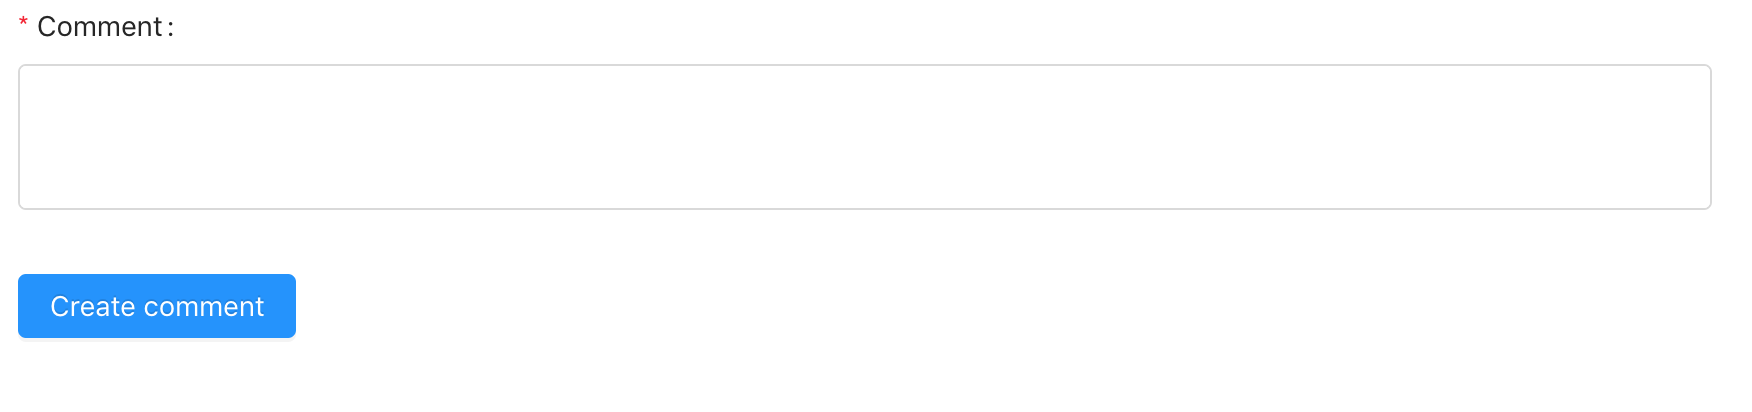
\includegraphics[width=\linewidth]{images/komentarz.png}
    \caption{Formularz komentarzy}
    \label{fig:comment}
\end{figure}

\subsection{Obszar powiadomień}
W obszarze powiadomień (rys. \ref{fig:notification}) użytkownik ma dostęp do listy swoich powiadomień pochodzących między innymi z komentarzy.
\begin{figure}[H]
    \centering
    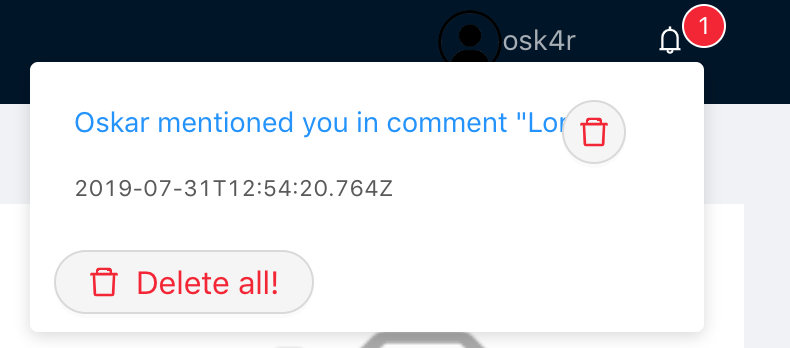
\includegraphics[width=\linewidth]{images/powiadomienia.png}
    \caption{Ekran obszaru powiadomień}
    \label{fig:notification}
\end{figure}


\chapter{Podsumowanie}
Celem pracy było utworzenie platformy blogowej łączącej funkcje serwisów Reddit i Medium. Do implementacji użyto nowoczesnych narzędzi takich jak frameworki React i Ruby on Rails. Pozwoliło to stworzyć aplikację spełniającą nowoczesne standardy programistyczne oraz standardy z zakresu interfejsu użytkownika. System dzięki zastosowanym w nim technologiom i architekturze umożliwia dalszy rozwój.

\section{Dalszy rozwój}

Biorąc pod uwagę skalę popularności serwisów o podobnej funkcjonalności, można stwierdzić, że w wyniku dalszego rozwoju aplikacji będzie ona mogła zostać wprowadzona na rynek komercyjny. Aby zwiększyć częstotliwość korzystania z serwisu, przydatny może być system powiadomień. Jego rozbudowa o nowe typy notyfikacji sprawi, że odbiorcy częściej będą odwiedzać portal. W celu wizualnego uatrakcyjnienia serwisu przydatną funkcją będzie rozbudowa edytora wpisów o możliwość pogrubiania czcionki, stosowania kursywy czy zmiany wielkości czcionki. Należy wziąć pod uwagę, że nie każdy użytkownik jest zainteresowany wszystkimi treściami. Trzeba rozważyć wprowadzenie możliwości personalizacji strony głównej przez wybór kategorii, z jakich mają być wyświetlane wiadomości. Dzięki zastosowanej architekturze oddzielającej część serwerową od interfejsu użytkownika istnieje możliwość, aby w przyszłości powstała aplikacja mobilna wykorzystująca React Native oraz już istniejące API.


%%%%% BIBLIOGRAFIA

\begin{thebibliography}{99}
\bibitem{reddit} Reddit
\url{https://www.redditinc.com/}
\bibitem{medium} Medium
\url{https://medium.com/}
\bibitem{twitter} Twitter
\url{https://twitter.com/}

\bibitem{facebook} Facebook
\url{https://www.facebook.com}
\bibitem{wykop} Wykop.pl 
\url{https://www.wykop.pl}
\bibitem{ruby} Ruby
\url{https://www.ruby-lang.org/}
\bibitem{ror} Ruby on Rails
\url{https://rubyonrails.org/}
\bibitem{postgre} PostgreSQL
\url{https://www.postgresql.org/}
\bibitem{react} React
\url{https://reactjs.org/}
\bibitem{bundler} Bundler
\url{https://bundler.io/}
\bibitem{foreman} Foreman
\url{https://github.com/ddollar/foreman}
\bibitem{redis} Redis
\url{https://redis.io/}
\bibitem{yarn} Yarn
\url{https://yarnpkg.com/lang/en/}
\bibitem{rorwiki} Ruby on Rails
\url{https://en.wikipedia.org/wiki/Ruby_on_Rails}
\bibitem{coc} Convention Over Configuration
\url{https://en.wikibooks.org/wiki/Ruby_on_Rails/Getting_Started/Convention_Over_Configuration}
\bibitem{dry} Don't repeat yourself
\url{https://en.wikipedia.org/wiki/Dont_repeat_yourself}
\bibitem{django} Django
\url{https://www.djangoproject.com/}
\bibitem{sails} Sails.js
\url{https://sailsjs.com}
\bibitem{rortutorial} Ruby on Rails: 
Getting Started with Rails
\url{https://guides.rubyonrails.org/getting_started.html}
\bibitem{sql2011} SQL:2011 
\url{https://www.iso.org/standard/53681.html}
\bibitem{acid} ACID
\url{https://en.wikipedia.org/wiki/ACID}
\bibitem{sidekiq} Sidekiq
\url{https://github.com/mperham/sidekiq}
\bibitem{ci} Continuous integration
\url{https://en.wikipedia.org/wiki/Continuous_integration}
\bibitem{travis} Travis CI
\url{https://travis-ci.org}
\bibitem{reactwiki}
\url{https://en.wikipedia.org/wiki/React_(web_framework)}
\bibitem{reactnative} React Native
\url{https://facebook.github.io/react-native/}
\bibitem{ant} Ant Design
\url{http://ant.design}
\bibitem{cra} Create React App
\url{https://github.com/facebook/create-react-app}
\bibitem{reactrouter} React Router
\url{https://reacttraining.com/react-router/web/guides/quick-start}
\bibitem{hooks} React: Introducing Hooks
\url{https://reacttraining.com/react-router/web/guides/quick-start}
\bibitem{token} Devise token auth: Conceptual diagrams
\url{https://devise-token-auth.gitbook.io/devise-token-auth/conceptual}

\end{thebibliography}

\end{document}